% !TEX encoding = UTF-8 Unicode
%Präambel

%Report für große Doukumente. Dieser ist in Kapitel (\chapter{}) aufgeteilt
%\documentclass[12pt, a4paper, ngerman]{report} 

%Article für normale Doumente
\documentclass[12pt, a4paper, ngerman]{article}

%Deutsche Beschreibungen von generiertem Text (table of contents => Inhaltsverzeichnis)
\usepackage[ngerman]{babel}

%Umlaute
\usepackage[utf8]{inputenc}

%Schriftart Helvetica 
\usepackage[scaled]{helvet}

%Seitenränder
\usepackage{geometry}
%top = Abstand nach oben
%left = Abstand nach links
%right = Abstand nach rechts
%bottom= Abstand nach unten
%heapsep= Abstand zwische Kopfzeile und Text
%footskip= Abstand zwischen Text und Fußzeile
\geometry{a4paper, top=25mm, left=30mm, right=25mm, bottom=30mm, headsep=10mm, footskip=12mm}

%Farben nutzen
\usepackage{xcolor}

%Grafiken einbinden
\usepackage{graphicx}

%Zusätzliche Positionsbefehle
\usepackage{float} 

%Die Einrücktiefe bei einem neuen Absatz
\setlength{\parindent}{0pt}

%Fülltext
\usepackage{blindtext}


%Fuer Zitate	
\PassOptionsToPackage{backend=bibtex}{biblatex}
\usepackage[natbib=true,style=numeric]{biblatex}
\usepackage[babel,german=guillemets]{csquotes}
\bibliography{quellen.bib} 

% Aufnahme von \paragraph in das Inhaltsverzeichnis 
\setcounter{tocdepth}{3}  

%Nummerierung vertiefen, \paragraph kommt mit ins Inhaltsverzeichnis
\setcounter{secnumdepth}{4} 

%Feste Tabellen
\usepackage{tabulary}

%caption für nummerierte Tabellenüberschriften
%booktabs für die Steuerung von Linien
\usepackage{caption, booktabs}

%Package fuer Use Cases
\usepackage{useCases}

%Package, um Attribute zu beschreiben
\usepackage{attribute}

%Package, um PDF Dokumente einzubinden
\usepackage{pdfpages} 


%Eigene Kommandos

\newcommand{\todo}[1]{\fcolorbox{red}{yellow}{ \parbox{0.75\linewidth}{#1}}} %To mark tasks can be done, but are not done 
\newcommand{\later}[1]{\fcolorbox{red}{orange}{\parbox{0.75\linewidth}{#1}}} %To mark tasks in the future. Can't be done now (e.g. missing information)
\newcommand{\checked}[1]{\fcolorbox{green}{green}{\parbox{0.75\linewidth}{#1}}} %To mark tasks, containing checked information
\newcommand{\crap}[1]{\fcolorbox{red}{red}{\parbox{0.75\linewidth}{#1}}} %To mark tasks, being absolutely bullshit

\begin{document}

\tableofcontents 
\newpage

\section{Einleitung}

\section{Use Cases}
Im Folgenden wird beschrieben, welche Use Cases das Programm in seiner Release Version bedienen kann.
\begin{figure}[htbp] 
  \centering
     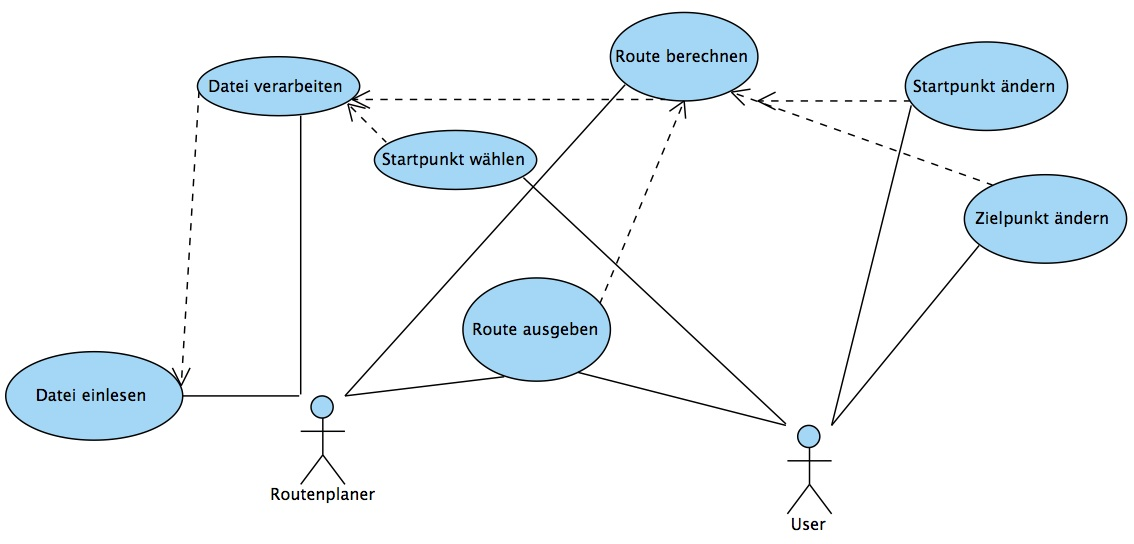
\includegraphics[width=0.9\textwidth]{Grafiken/primaryUseCases.jpg}
  \caption{Übersicht über die Use Cases}
  \label{fig:uebersichtUseCases}
\end{figure}

\subsection{Automatischer Ablauf}
\subsubsection{Datei einlesen \label{uc:DateiEinlesen}}
\begin{usecase}
	\utitle{Datei einlesen}
	\udescription{Nachdem das Programm gestartet wird, wird die csv Datei mit den Streckeninformationen eingelesen.}
	\uactor{Routenplaner}
	\utrigger{Der Start des Programms}
	\uprecondition{Eine gültige Datei mit den Streckeninformationen muss vorliegen, Der richtige Dateiname und -Pfad muss im Programm angegeben sein}
	\upostcondition{Der Inhalt der Datei befindet sich im Arbeitsspeicher}
\end{usecase}

\subsubsection{Datei verarbeiten \label{uc:DateiVerarbeiten}}
\begin{usecase}
	\utitle{Datei verarbeiten}
	\udescription{Aus der bereits eingelesenen Datei werden Objekte erstellt.}
	\uactor{Routenplaner}
	\utrigger{Die Verarbeitung Use Case \ref{uc:DateiEinlesen} ist abgeschlossen}
	\uprecondition{Use Case \ref{uc:DateiEinlesen}}
	\upostcondition{Die primäre Funktionalität des Routenplaners steht dem User zur Verfügung}
\end{usecase}

\subsubsection{Distanzen berechnen \label{uc:RouteBerechnen}}
\begin{usecase}
	\utitle{Distanzen berechnen}
	\udescription{Der Routenplaner berechnet die kürzesten Wege vom Startpunkt zu allen anderen Punkten}
	\uactor{Routenplaner}
	\utrigger{Use Case \ref{uc:StartpunktWaehlen}} 
	\uprecondition{Use Case \ref{uc:DateiVerarbeiten}}
	\upostcondition{Die Distanzen vom Startpunkt zu allen anderen anderen Punkten sind bekannt}
\end{usecase}
\subsection{Abläufe, die vom User angestoßen werden}
\subsubsection{Startpunkt wählen \label{uc:StartpunktWaehlen}}
\begin{usecase}
	\utitle{Startpunkt wählen}
	\udescription{Der User wählt den Startpunkt der Routenberechnung aus}
	\uactor{User}
	\uprecondition{Use case \ref{uc:DateiVerarbeiten}, Der Startpunkt ist ein gültiger Punkt}
	\upostcondition{Die Route wird berechnet}
\end{usecase}

\subsubsection{Startpunkt ändern \label{uc:StartpunktAendern}}
\begin{usecase}
	\utitle{Startpunkt ändern}
	\udescription{Der User ändert den Startpunkt einer bereits berechneten Route}
	\uactor{User}
	\uprecondition{Use case \ref{uc:DateiVerarbeiten}, Der Startpunkt ist ein gültiger Punkt}
	\upostcondition{Die Route wird neu berechnet}
\end{usecase}

\subsubsection{Zielpunkt ändern \label{uc:ZielpunktAendern}}
\begin{usecase}
	\utitle{Zielpunkt ändern}
	\udescription{Der User trägt einen Zielpunkt ein, bzw. ändert einen bestehenden. }
	\uactor{User}
	\uprecondition{\ref{uc:RouteBerechnen}}
	\upostcondition{Der Routenplaner sucht die kürzeste Route und gibt diese aus (Use Case \ref{uc:RouteAusgeben})}
\end{usecase}

\subsubsection{Route ausgeben \label{uc:RouteAusgeben}}
\begin{usecase}
	\utitle{Route ausgeben}
	\udescription{Die kürzeste Route vom Start- zum Zielpunkt wird ausgegeben}
	\uactor{Routenplaner}
	\uprecondition{Use Case \ref{uc:RouteBerechnen},Use Case \ref{uc:ZielpunktAendern}}
\end{usecase}

\section{Verarbeitete Daten}
Der Routenplaner verarbeitet sämtliche Daten, die im Datensatz vorhanden sind. Da ein Großteil dieser Daten für die Verarbeitung optional ist, werden die notwendigen Daten mit \textit{mandatory} und die optionalen Daten mit \textit{optional} gekennzeichnet. Der Hintergrund, dass die optionalen Daten verarbeitet werden ist, dass optionalen Daten für eine informative Ausgabe benötigt werden können und dem User mehr Komfort bei der Ausgabe bieten können. Die optionalen Daten sind permanent vorhanden und können jederzeit im User Interface abgegriffen und ausgegeben werden.
Die Abbildung \ref{fig:klassendiagrammLokations} zeigt die Hierarchie der Lokationen und deren Attribute.

\begin{figure}[htbp] 
  \centering
     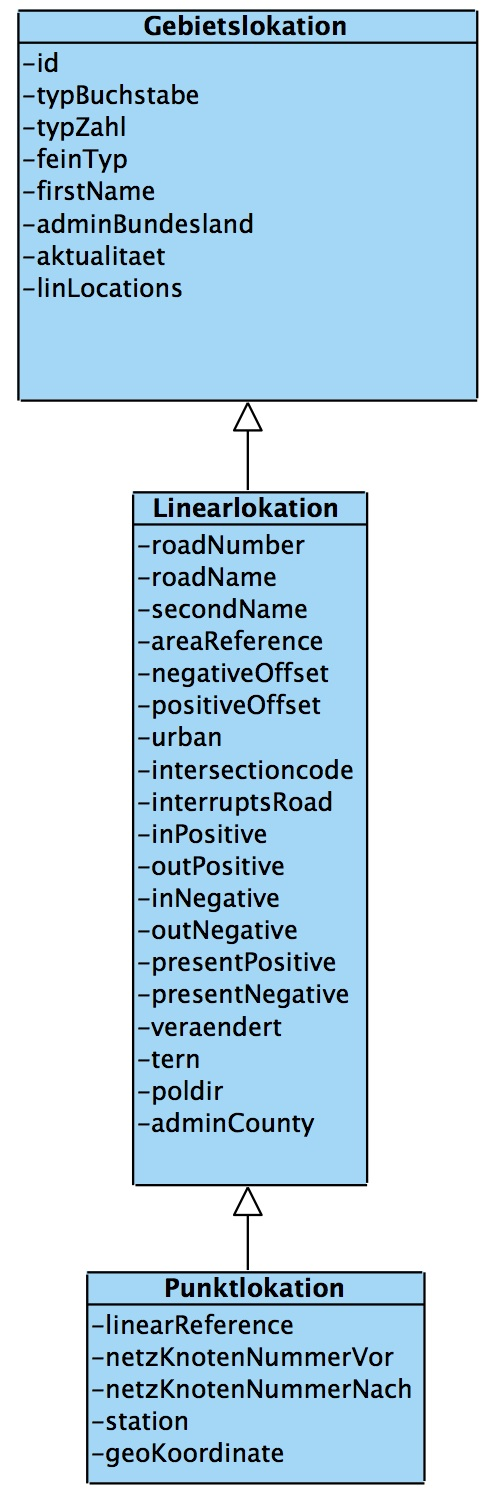
\includegraphics[width=0.3\textwidth]{Grafiken/klassenDiagrammLokations.jpg}
  \caption{Aufbau der Lokations}
  \label{fig:klassendiagrammLokations}
\end{figure}

Der originale Datensatz wurde in drei Klassen nachgebildet. Diese entsprechen auch den verschiedenen Location, die in der original Dokumentation des Bundes beschrieben sind.
\subsection{Area Location \label{AreaLocation}}
Eine Area Location, oder Gebietslokation, ist ein grobes Gebiet. Gebiete können beispielsweise Kontinente, Länder, Bundesländer oder Ballungsgebiete sein. Sie stellt den Grundtyp der anderen Lokalionen dar.

\begin{attribut}{Id}
	\drequried{ja}
	\dtype{unsigned int}
	\dmapping{LOCATIONCODE}{Id}
	\dbeschreibung{Eine Id ist einer Lokation eindeutig zugeordnet. Sie wird mit aus dem Datensatz ausgelesen und fest mit dem Objekt verbunden.}
\end{attribut}

\begin{attribut}{typBuchstabe}
	\drequried{nein}
	\dtype{char}
	\dmapping{TYPE}{typBuchstabe + typZahl}
	\dbeschreibung{Dieses Attribut gibt an, um welchen Typ von Lokation es sich handelt. Der ursprüngliche Datentyp besteht aus der Kombination \textless Art der Lokation\textgreater \textless Beschreibung\textgreater. Die Art der Lokation ist ein Buchstabe, der in diesem Attribut gespeichert wird.}
	\dbelegung{A - Gebietslokation, L - Linearlokation, P - Punktlokation }
\end{attribut}

\begin{attribut}{typZahl}
	\drequried{nein}
	\dtype{int}
	\dmapping{TYPE}{typBuchstabe + typZahl}
	\dbeschreibung{Dieses Attribut beschreibt die Lokation genauer. Der ursprüngliche Datentyp besteht aus der Kombination \textless Art der Lokation\textgreater \textless Beschreibung\textgreater. Die genauere Beschreibung der Lokation ist eine Zahl.}
	\dbelegung{1 - Kontinent, 2 - Ländergruppe, 3 - Land, 5 - Wasser, 6 - Allgemeines Gebiet, 7 - Bundesland}
\end{attribut}
Die Beschreibung von Lokationen kann weiter herunter gebrochen werden. Die Beschreibung, welche Zahlenwerte hierfür zur Verfügung stehen findet im angehängten Dokument unter \ref{bundFeinDoku}.
\subsection{Linearlokation}
\later{TypZahl dokumentieren}

\section{Anhang}
\subsection{Typen und Untertypen der Lokationen \label{bundFeinDoku}}

\includepdf[pages={1-14}]{Grafiken/RelatedDocuments/Typenliste_V08_2010-03-03.pdf}
\end{document}